%\documentclass[a4paper,10pt]{article}
\documentclass[10pt, conference, letterpaper]{algotel}
\usepackage[utf8]{inputenc}
\usepackage{xspace}
\usepackage{url}
\usepackage{graphicx,graphics} 
\usepackage{color}
\usepackage{amsmath}
\usepackage{amsfonts}
\usepackage{amssymb}
\usepackage{amsthm}
\usepackage{algorithm}
\usepackage{algorithmic}
\usepackage{longtable}
\usepackage{complexity}
\usepackage{tkz-graph}
\usepackage{float}
\usepackage{tabularx}
\usepackage{setspace}
\usepackage{icomma}
\usepackage{tkz-graph}
\usepackage{complexity}
\renewcommand{\algorithmicrequire}{\textbf{Input:}}
\renewcommand{\algorithmicensure}{\textbf{Output:}}
\usepackage[colorlinks=true,breaklinks=true,linkcolor=blue]{hyperref}


\newtheorem{proposition}{Proposition}
\newtheorem{theorem}{Theorem}

\setlength{\parskip}{1ex} % Espace entre les paragraphes

\newtheorem{fact}{Fact}
\newtheorem{lemma}[theorem]{Lemma}
\newtheorem{definition}{Definition}
\newtheorem{corollary}{Corollary}

% \renewcommand{\thefootnote}{\*}

\newcommand\pma{\textsc{pma}\xspace}
\newcommand{\todo}[1]{{\color{red} TODO: {#1}}}
\title{Scheduling periodic messages on a shared link}
 

\author[1,2]{Ma\"el Guiraud}
\author[1]{Yann Strozecki}
\affil[1]{David Laboratory, UVSQ}
\affil[2]{Nokia Bell Labs France}

\begin{document}

\maketitle

%En français
%Ordonnancement de messages périodiques et de leurs réponses sur un lien partagé

%Le Cloud-RAN est une nouvelle architecture de réseau mobile dans laquelle les unités de calcul, traditionnellement 
% installées au pieds des antennes, sont déportées dans des data-centers distants. Dans ces conditions, pour respecter des contraintes liées aux protocoles 4G et 5G, il faut minimiser la latence des messages périodiques envoyés par les antennes
%à leurs unités de calcul. Nous essayons donc ici de trouver des plans périodiques de transmission des messages qui ne nécessitent pas de buffer et donc de latence supplémentaire.

%Dans cet article nous étudions une topologie en étoile, ou la contention vient d'un lien partagé entre toutes les antennes.
%Pour des messages arbitrairement grand, nous montrons qu'il existe toujours un plan de transmission des messages si la charge du réseau est inférieure à $40\%. De plus, nous montrons comment réduire le problème à des messages de taille unitaire
%pour une latence additionnelle modeste.

%Pour les messages de taille $1$, nous donnons un algorithme en temps polynomial qui trouve un plan de transmission
%pour des charges jusqu'à $58\%$. De plus, en analysant un algorithme aléatoire glouton, pour n'importe quelle charge, 
% presque toutes les instances avec suffisamment de messages ont une solution, ce qui explique pourquoi les algorithmes
%gloutons présentés dans l'article marchent si bien en pratique.


%keywords :C-RAN; latency; periodic scheduling; greedy algorithms


\begin{abstract}
Cloud-RAN is a recent architecture for mobile networks where the processing units are located in distant data-centers while, until now, they were attached to antennas. The main challenge, to fulfill protocol time constraints, is to guarantee a low latency for the periodic messages sent from each antenna to its processing unit and back. The problem we address is to find a sending scheme of these periodic messages without contention nor buffering.

We focus on a simple but common star shaped topology, where all contentions are on a single link shared by all antennas. For messages of arbitrary size, we show that there is always a solution as soon as the load of the network is less than $40\%$.
For message of size $1$, we prove that it is always possible to schedule them, when the load is less than $61\%$  using a polynomial time algorithm. Moreover, using a simple random greedy algorithm, we show that almost all instances of a given load admit a solution, explaining why most greedy algorithms work so well in practice.  
\end{abstract}

\section{Introduction and model}

Next generations of mobile network architectures evolve toward centralized radio network architectures called C-RAN for Cloud Radio Access Network, to reduce energy consumption costs~\cite{mobile2011c} and more generally the total cost of ownership. The main challenge for this type of architecture is to reach a latency compatible with transport protocols~\cite{ieeep802}. The specificity of the C-RAN context is not only the latency constraint, but also the periodicity of the data transfer in the frontaul network between RRHs and BBUs: messages need to be emitted and received each millisecond~\cite{bouguen2012lte}. Our aim is to operate a C-RAN on a low-cost shared switched network. 

 Statistical multiplexing even with a large bandwidth does not satisfies the latency requirements of C-RAN~\cite{dominique2018deterministic,barth2018deterministic}. The current solution~\cite{pizzinat2015things,tayq2017real} is to use dedicated circuits for the fronthaul. Each end-point, an RRH on one side and a BBU on the other side is connected through direct fiber or full optical switches. This eliminates all contentions since each message flow has its own link, but it is extremely expensive and do not scale in the case of a mobile network composed of about $10,000$ base stations. 

The question we address is the following: \emph{is it possible to schedule periodic messages on a shared link without using buffers}? Eliminating this source of latency leaves us with more time budget for latency due to the physical length of the routes in the network, and thus allows for wider deployment areas. Our proposed solution is to compute beforehand a \emph{periodic and deterministic} sending scheme, which completely avoids contention. This kind of deterministic approach has gained some traction recently: Deterministic Networking is under standardization in IEEE 802.1 TSN group~\cite{finn-detnet-architecture-08}, as well at IETF DetNet working group~\cite{ieee802}.

We now formally describe our model and problem.
The time is discretized and the process we consider is periodic of fixed integer period $P$. We use the notation $[P]$ for the set $\{0,\dots,P-1\}$. In the C-RAN network we model, all messages are of the same nature, hence they are all of the same size denoted by $\tau$. This size corresponds to the time needed to send a message through some contention point of the network, here a link shared by all antennas. We denote by $n$ the number of messages, which are numbered from $0$ to $n-1$. A message $i$ is characterized by its delay $d_i$. It means that if the message number $i$ arrives at the link at time $t$, then it returns to the other end of the link on its way back at time $t + d_i$. 

Since the process we describe is periodic, we may consider any interval of $P$ units of time
to represent the state of our system. Describing the messages going through the two contention points during such an interval completely defines the periodic process. We call the representation of the interval of time in the first contention point the \emph{first period} and the \emph{second period} for the second contention point.

An \emph{offset} of a message is a choice of time at which it arrives
at the first contention point. Let us consider a message $i$
of offset $o_i$, it uses the interval of time $[i]_1 = \{ (o_i + t) \mod P \mid 0 \leq t < \tau \}$ in the first period and $[i]_2 = \{ (d_i + o_i + t) \mod P \mid 0 \leq t < \tau \}$ in the second period. We say that two messages $i$ and $j$ collide if either $[i]_1 \cap [j]_1 \neq \emptyset $ or $[i]_2 \cap [j]_2 \neq \emptyset $. If $t \in [i]_1$ (resp. $t \in [i]_2$) we say that message $i$ uses time $t$ in the first period (resp. in the second period).

We want to send all messages, so that they are no collision in the shared link.
In other word, we look for a way to send the messages without using buffering and 
hence limiting the latency to the physical length of the links. An assignment is a
choice of an offset for each message such that \emph{no pair of message collide}, as shown in Fig.~\ref{fig:assignment}. Formally, an \emph{assignment} is a function from the messages in $[n]$ to their offsets in $[P]$.  

We call Periodic Message Assignment or \pma the problem studied in this article,
which asks, given an instance of $n$ messages, a period $P$ and a size $\tau$, to find 
an assignment or to decide there is none.
\begin{figure}
\begin{center}
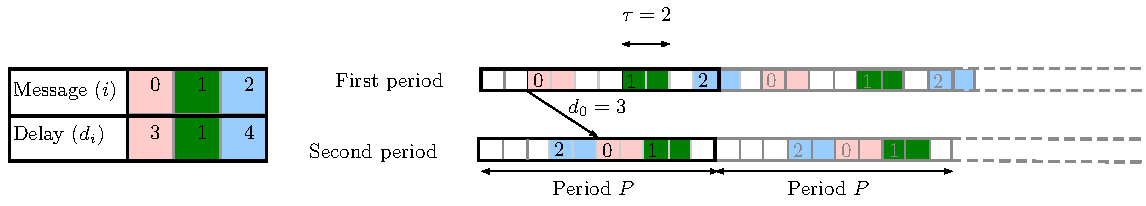
\includegraphics[scale=0.7]{instance}
\end{center}
\caption{An instance of \pma ($n=3$, $P= 10$, $\tau = 2$) and one assignment}
\label{fig:assignment}
\end{figure}




In previous articles of the authors, generalizations of \pma allowing buffers are studied on a single link~\cite{dominique2018deterministic} or on a cycle~\cite{Guir1905:Deterministic}. Heuristics (using scheduling algorithms) and FPT algorithms are used to find a sending scheme with \emph{minimal latency}, while here we only look for sending scheme without any additional latency. More complex problems of computing schedules for time sensitive networks, such as sensor networks inside a car or a plane, have been practically solved~\cite{nayak2017incremental,steiner2018traffic,dos2019tsnsched}. 

\pma is similar to the two flow shop scheduling problem~\cite{yu2004minimizing}, 
but the \emph{periodicity} modifies it fundamentally: messages from consecutive periods can interact and the objective is quite different from makespan minimization.
Periodic scheduling have also been studied, but to our knowledge the problems are quite different from \pma. Often, the aim is to minimize the number of processors on which the periodic tasks are scheduled~\cite{korst1991periodic,hanen1993cyclic}, while \pma corresponds to a single processor and a constraint similar to makespan minimization. In cyclic scheduling~\cite{levner2010complexity}, the aim is to minimize the period of a scheduling to maximize the throughput, while our period is fixed. The train timetabling problem~\cite{lusby2011railway} and in particular the periodic event scheduling problem~\cite{serafini1989mathematical} are generalizations of our problem. However, they are much more general~\cite{lusby2011railway}: the trains can vary in size, speed, the network can be more complex than a single track and there are precedence constraints.


The complexity of \pma is not yet known. However, we have proven that, when parameterized by
$n$ the number of messages, the problem is \FPT~\cite{barth2018deterministic}.
A slight generalization of \pma, with several contention points but each message only going through two of them, as in \pma, is \NP-hard~\cite{barth2018deterministic}. If the shared link is not bidirectional, that is there is a single contention point and each message goes through it twice, it is also \NP-hard~\cite{orman1997complexity}. Hence, we conjecture that \pma is \NP-hard.

To overcome the supposed hardness of \pma, we study it when the load of the system is small enough. The \emph{load} is defined as the number of units of time used in a period by all messages divided by the period. Hence the load is equal to $n\tau /P$. Our aim is to prove that, for small load, there is \emph{always} an assignment and that it can be found by a polynomial time algorithm.


\section{Greedy Algorithms for Large Messages} \label{sec:large}

In this section, we study the case of large messages. When modeling real problems,
it is relevant to have $\tau > 1$ when the transmission time of a single message is large with regard to its delay.

A partial assignment $A$ is a function defined from a subset $S$ of $[n]$ to $[P]$.
We say that $|S|$, the cardinal of the domain of $A$, is its \emph{size}.
We say that a message in $S$ is \emph{scheduled} (by $A$), and a message not in $S$ is \emph{unscheduled}. We only consider partial assignments such that no pair of messages of $S$ collide. If $A$ has domain $S$, and $i \notin S$, we define the extension of $A$ to the message $i$ by the offset $o$, denoted by $A[i \rightarrow o]$, the function defined as $A$ on $S$ and $A[i \rightarrow o](i) = o$.


\subsection{First Fit}


Let $Fo(A)$ be the maximum number of forbidden offsets when extending $A$ by some route. Formally, assume $A$ is defined over $S$ and $i\notin S$, $Fo(A)$ is the maximum over all values of $d_i$ of $|\left\{ o \in [P] \mid A[i \rightarrow o] \text{ has no collision }\right\}|$.
A simple analysis shows that $|S|$ scheduled routes forbid $(2 \tau -1)|S|$ offsets because of the times used in the first period and $(2 \tau -1)|S|$ offsets because of the times used in the second period. Hence, $Fo(A)$ is always bounded by $(4 \tau -2)|S|$.  Remark that if $Fo(A) < P$, then whatever the delay of the route we want to extend $A$ with, it is possible to find an offset. Since $Fo(A) \leq (4 \tau -2)|S|$ and $|S| < n$,  any greedy algorithm will always succeed when $(4 \tau -2)n \leq P$, that is when the load $ n\tau /P$ is less than $1/4$.


The \emph{First Fit} algorithm deals with the route in the order they are given:  for each unscheduled route it tests all offsets from $0$ to $P-1$ until one do not create a collision with the current assignment. It turns out that First Fit always creates compact assignments (as defined in~\cite{dominique2018deterministic}), that is a message is always next to another one in one of the two period, which yields a better bound on $Fo(A)$ and implies the following theorem.

\begin{theorem}
First Fit always solves \pma positively on instances of load less than $1/3$. 
\end{theorem}


\subsection{Meta-Offset}

The second method is described  in~\cite{dominique2018deterministic} and achieves the same bound on the load using a different method.
The idea is to restrict the possible offsets at which messages can be scheduled to reduce the number of forbidden offsets on the first period. A \emph{meta-offset} is an offset of value $i\tau$, with $i$ an integer from $0$ to $P / \tau$. We call Meta-Offset the greedy algorithm
which works as First Fit, but consider only meta-offsets when scheduling new messages. 

Let $Fmo(A)$ be the maximal number of meta-offsets forbidden by $A$. 
 By definition, two messages with a different meta-offset cannot collide in the first period.
Hence, $Fmo(A)$ can be bounded by $3|S|$ and we obtain the following theorem.


\begin{theorem}[Proposition 3 of~\cite{dominique2018deterministic}]
Meta-Offset always solves \pma positively on instances of load less than $1/3$.
\end{theorem}

\subsection{Tuples and meta-intervals}

We now propose a more involved family of greedy algorithms which 
solves \pma positively for larger loads. We try to combine the good properties of the two previous algorithms: the compacity of the assignments produced by First Fit and the use of meta-offsets to reduce collisions on the first period. The idea is to schedule several messages at once, using meta-offsets, to maximize the compacity of the obtained solution. 

We first states a lemma which allows to assume that the period $P$ is a multiple of $\tau$, since it makes the analysis of our algorithms much simpler and tighter. It only changes the load from $n \tau / P$ to at most $n (\tau +1)/ P$: the difference is less than $n /P < 1/\tau$, and thus very small for large $\tau$.

\begin{lemma}
Let $I$ be an instance of \pma with $n$ messages of size $\tau$, period $P$ and $m = P / \tau$. There is an instance $I'$ with $n$ messages of size $\tau'$ and period $P'= m\tau'$ such that an assignment of $I'$ can be transformed into an assignment of $I$ in polynomial time.
\end{lemma}

From now on, we always assume that $P = m\tau$ and the load is then $n/m$.
We are interested in the remainder modulo $\tau$ of the delays of each message.
We write $d_i = d_{i}'\tau + r_i$ and assume from now on that messages are sorted by increasing $r_i$.
A \emph{compact pair} is a pair of messages $(i,j)$ with $i < j$ such that we can put them next to each other in the second period using meta-offsets.
We have $r_i \leq r_j$ since $i < j$. We denote by $g$ the gap between the two messages in the first period, that we define by $d_{i}' = g + 1 + d_{j}' \mod m$. We require that $g \neq 0$ so that there are no collision in the first period if we schedule these two messages such that the difference of their offsets is the gap. 


\begin{lemma}\label{lemma:pair_find}
Given $3$ messages, two of them always form a compact pair. 
\end{lemma}

We call \emph{Compact Pairs} the following greedy algorithm. From the $n$ routes in order
of increasing $r_i$, we build a sequence of at least $n/3$ compact pairs using Lemma~\ref{lemma:pair_find}. They are then scheduled in the order they have been built using meta-offsets only. If at some point all compact pairs are scheduled or the current one cannot be scheduled, the remaining messages are scheduled as in Meta-Offset. The analysis of the algorithm relies on the evaluation of the number of forbidden meta-offsets. In the first phase of the algorithm, one should evaluate the number of forbidden offsets when scheduling a compact pair, that we denote by $Fmo_2(A)$. In the second phase, we need to evaluate $Fmo(A)$. When scheduling a message in the second phase, a scheduled compact pair only forbids \emph{three} meta-offsets in the second period. If messages in a pair are scheduled independently, they forbid \emph{four} meta-offsets, which explains the improvement from Meta Offset. We use a simple lemma, which allows to bound $Fmo_2(A)$.

\begin{lemma}\label{lemma:pair_forbid}
A compact pair already scheduled by Compact Pair forbids at most four meta offsets in the second period to another compact pair when it is scheduled by Compact Pair.
\end{lemma}

\begin{theorem}
Compact Pairs always solves \pma positively on instances of load less than
$3/8$.
\end{theorem}

The algorithm can be improved by forming compact $k$-tuples instead of compact pairs
from large $k$ down to $2$. It works when the load is less than $4/10$, see~\cite{}. 


\subsection{Experimental Results} \label{sec:perf_large}

We present results of simulations of the algorithms presented above, to experimentally assess their performance on random instances (code on \url{https://yann-strozecki.github.io/}). The parameters are $P = 100000$, $\tau = 1000$ and instances of \pma are generated by drawing uniformly and independently the delays of each message in $[P]$.
The success rate for each load is measured on $10000$ random instances. In addition to the three presented algorithms, we also test Greedy Uniform wich builds greedily an assignment by randomly choosing possible offsets(see Sec.~\ref{sec:small}). Fig.\ref{fig:100messBig} shows that all algorithms performs better than the worst case bound given in the section. First Fit performs better than Meta Offset while they have the same worst case. Compact Pair, which is the best theoretically also performs the best in the experiment, always finding assignments for load of $0.6$. 

\begin{figure}
\begin{center}
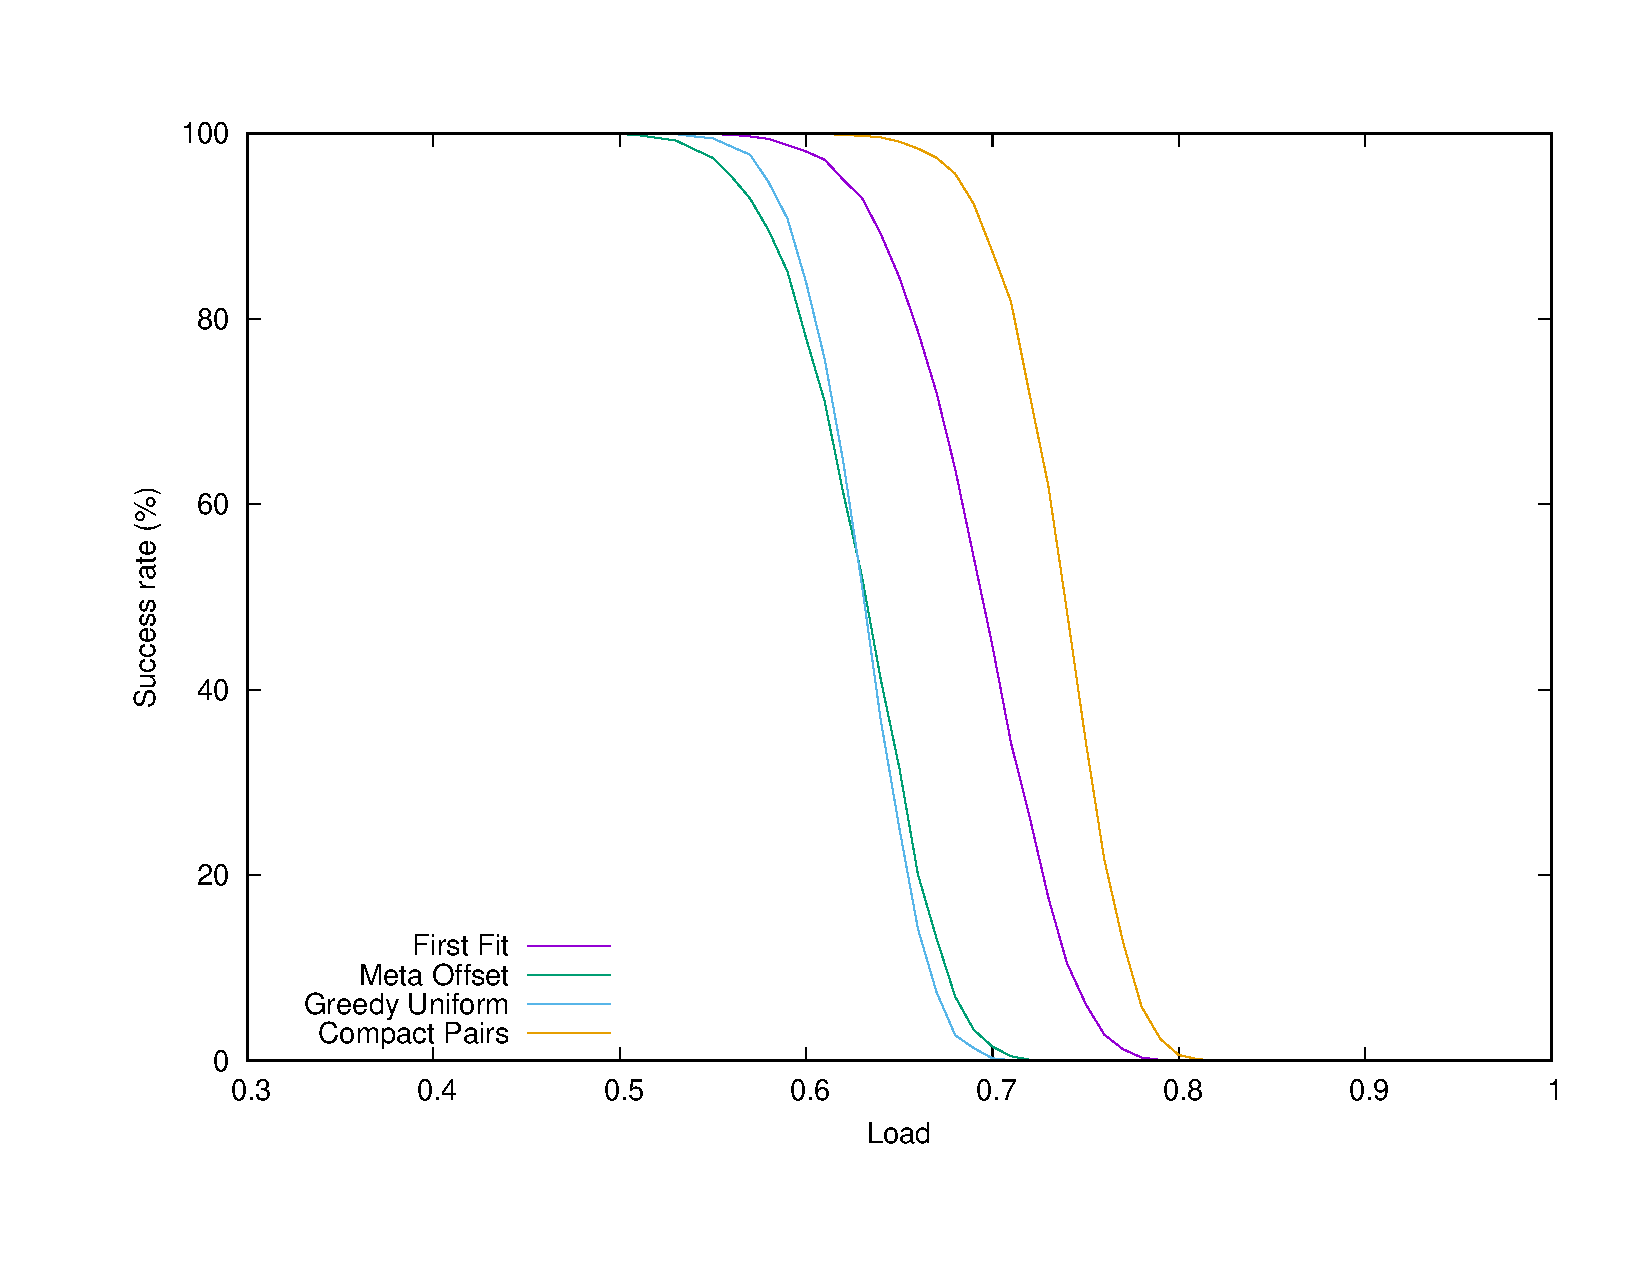
\includegraphics[scale=0.2]{100messBig}
\end{center}
\caption{Experiment for $\tau = 1000$, $P=100,000$}
\label{fig:100messBig}
\end{figure}

 \section{Messages of Size One} \label{sec:small}

When $\tau = 1$, \emph{any greedy algorithm} finds a solution to \pma when the load is less than $1/2$ since $Fo(A) \leq (4\tau -2)|S| = 2|S|$ where $S$ is the number of scheduled messages. We now give a method which always finds a solution for load of $1/2 + \epsilon$.

\subsection{Deterministic algorithm}

To go above $1/2$ of load, we use an algorithm which optimizes a potential measuring how many offsets are available for all messages, scheduled or not. Messages are scheduled while possible using any greedy algorithm.
Then, when all unscheduled messages have no free offset, we use a swap operation defined later, which improves the potential. When the potential is high enough, it ensures that there are two messages whose offset can be changed so that a new message can be scheduled. 
 

\begin{definition}
The potential of a message of delay $d$, for a partial assignment $A$
is the number of integers $i \in [P]$ such that $i$ is used in the first period and $i+d \mod P$ is used in the second period.
\end{definition}

The potential of a message counts favorable configurations in terms of forbidden offsets.
Indeed, when $i$ is used in the first period and $i+d \mod P$ is used in the second period,
then the same offset is forbidden \emph{twice} for a message of delay $d$. 
For our algorithm, we need a global measure of quality of a partial assignment, 
that we try to increase when the algorithm fail to schedule new messages. 
We call our measure \emph{the potential of an assignment} and we denote it by $Pot(A)$, it is the sum of potentials for $A$ of all messages in the instance.


\begin{definition}
The potential of a position $i$, for a partial assignment $A$, is the number of messages of delay $d$ such that $i+d \mod P$ is used by a route scheduled by $A$. 
\end{definition}

Instead of decomposing the global potential as a sum over the messages, it can be understood
as a sum over positions. Hence, the sum of potentials of all positions used in the first period by messages scheduled by $A$ is equal to $Pot(A)$.  Moreover, the sum of potentials of all positions for a partial assignment with $k$ scheduled messages is $nk$.  
In the algorithm we propose, we guarantee to obtain at last half this value by an exchange mechanism, that we call a swap. Let $A$ be some partial assignment of size $s$ and let $i$ be an unscheduled message of delay $d$. Assume that $i$ cannot be used to extend $A$. The swap operation is the following: 
select a free position $o$ in the first period, remove the message which uses the position $o+d$ in the second period from $A$ and extend $A$ by $i$ with offset $o$. We denote this operation by $Swap(i,o,A)$.

\begin{lemma}\label{lemma:swap}
Let $A$ be some partial assignment of size $k$ and let $i$ be an unscheduled message. If $i$ cannot be used to extend $A$, then either $Pot(A) \geq kn/2$ or there is an $o$ such that $Pot(Swap(i,o,A)) > Pot(A)$.
\end{lemma}


We now describe the \emph{Swap} algorithm. It schedules unscheduled messages while possible and then applies Swap operations while it increases the potential. When the potential is maximal, it tries to schedule a new message by moving one or two scheduled messages to new offsets. If it fails to find such messages the algorithm stops, otherwise it repeats the same steps. We now give an analysis of the algorithm, showing that it always works for a load small enough.

\begin{theorem}
The Swap algorithm solves positively \pma for instances with $\tau =1$ and load $1/2 + (\sqrt{5}/2 -1) \approx 0,618$.
\end{theorem}

\subsection{Random Algorithm for Random Instances}

We would like to understand better the behavior of our algorithms
on instances drawn uniformly at random. To this aim, we analyze the following algorithm, called \textbf{Greedy Uniform}: for each message in order, choose one of the possible offsets uniformly at random and use it to extend the partial assignment. 

We analyze Greedy Uniform over random instances: we assume that all messages have 
their delays drawn independently and uniformly in $[m]$. We compute the probability of success of Greedy Uniform over all random choices of the algorithm \emph{and all possible instances}. 
It turns out that this probability, for a fixed load strictly less than one, goes to one when $m$ grows. For a given assignment, we are only interested in its trace: the set of times which are used in the first and second period. Hence, if $n$ messages are scheduled in a period of size $m$, a trace of an assignment is a pair of subsets of $[m]$ of size $n$. We now show that these traces are produced uniformly.

\begin{theorem}
The distribution of traces of assignments produced by Greedy Uniform when it succeeds, from instances drawn uniformly at random, is also uniform.
\end{theorem}

Let $\Pr(m,n)$ be the probability that Greedy Uniform fails at the $n^{th}$ step assuming it has not failed before.

\begin{lemma}\label{lemma:proba_fail}
$$\Pr(m,n) = \frac{\binom{n}{2(n-1)-m}}{\binom{m}{n-1}}.$$
\end{lemma}

From Lemma~\ref{lemma:proba_fail}, we can derive the probability 
of success of Greedy Uniform by a simple product. 

\begin{theorem}\label{theorem:uniform}
The probability over all instances with $n$ messages and period $m$ that Greedy Uniform solves $\pma$ positively is $\displaystyle{\prod_{i=m/2}^{n-1}(1 - \frac{\binom{n}{2i-m}}{\binom{m}{i}})}$.
\end{theorem}

Let $\lambda$, be the load, we can prove using Stirling formula that
$P(m,n) C \lambda m f(\lambda)^m$ with $f(\lambda) < 1$. Thus, the probability that Greedy Uniform fails goes to $0$ when $m$ grows.

\subsection{Experimental results} \label{sec:perf_small}

 The settings are as in Sec.~\ref{sec:perf_large}, with $\tau = 1$ and 
 similarly, the success rate on random instances is much better than the worst case analysis.
As shown in Fig.~\ref{fig:tau1}, all algorithms succeed on all instances when the load is less than $0.64$. Greedy Uniform behaves exactly as proved in Theorem~\ref{theorem:uniform}, with a very small variance. Amazingly, Swap always finds an assignment when the load is less than $0.95$, but it is not always able to find assignments when compared to an exact resolution. 

\begin{figure}
\begin{center}
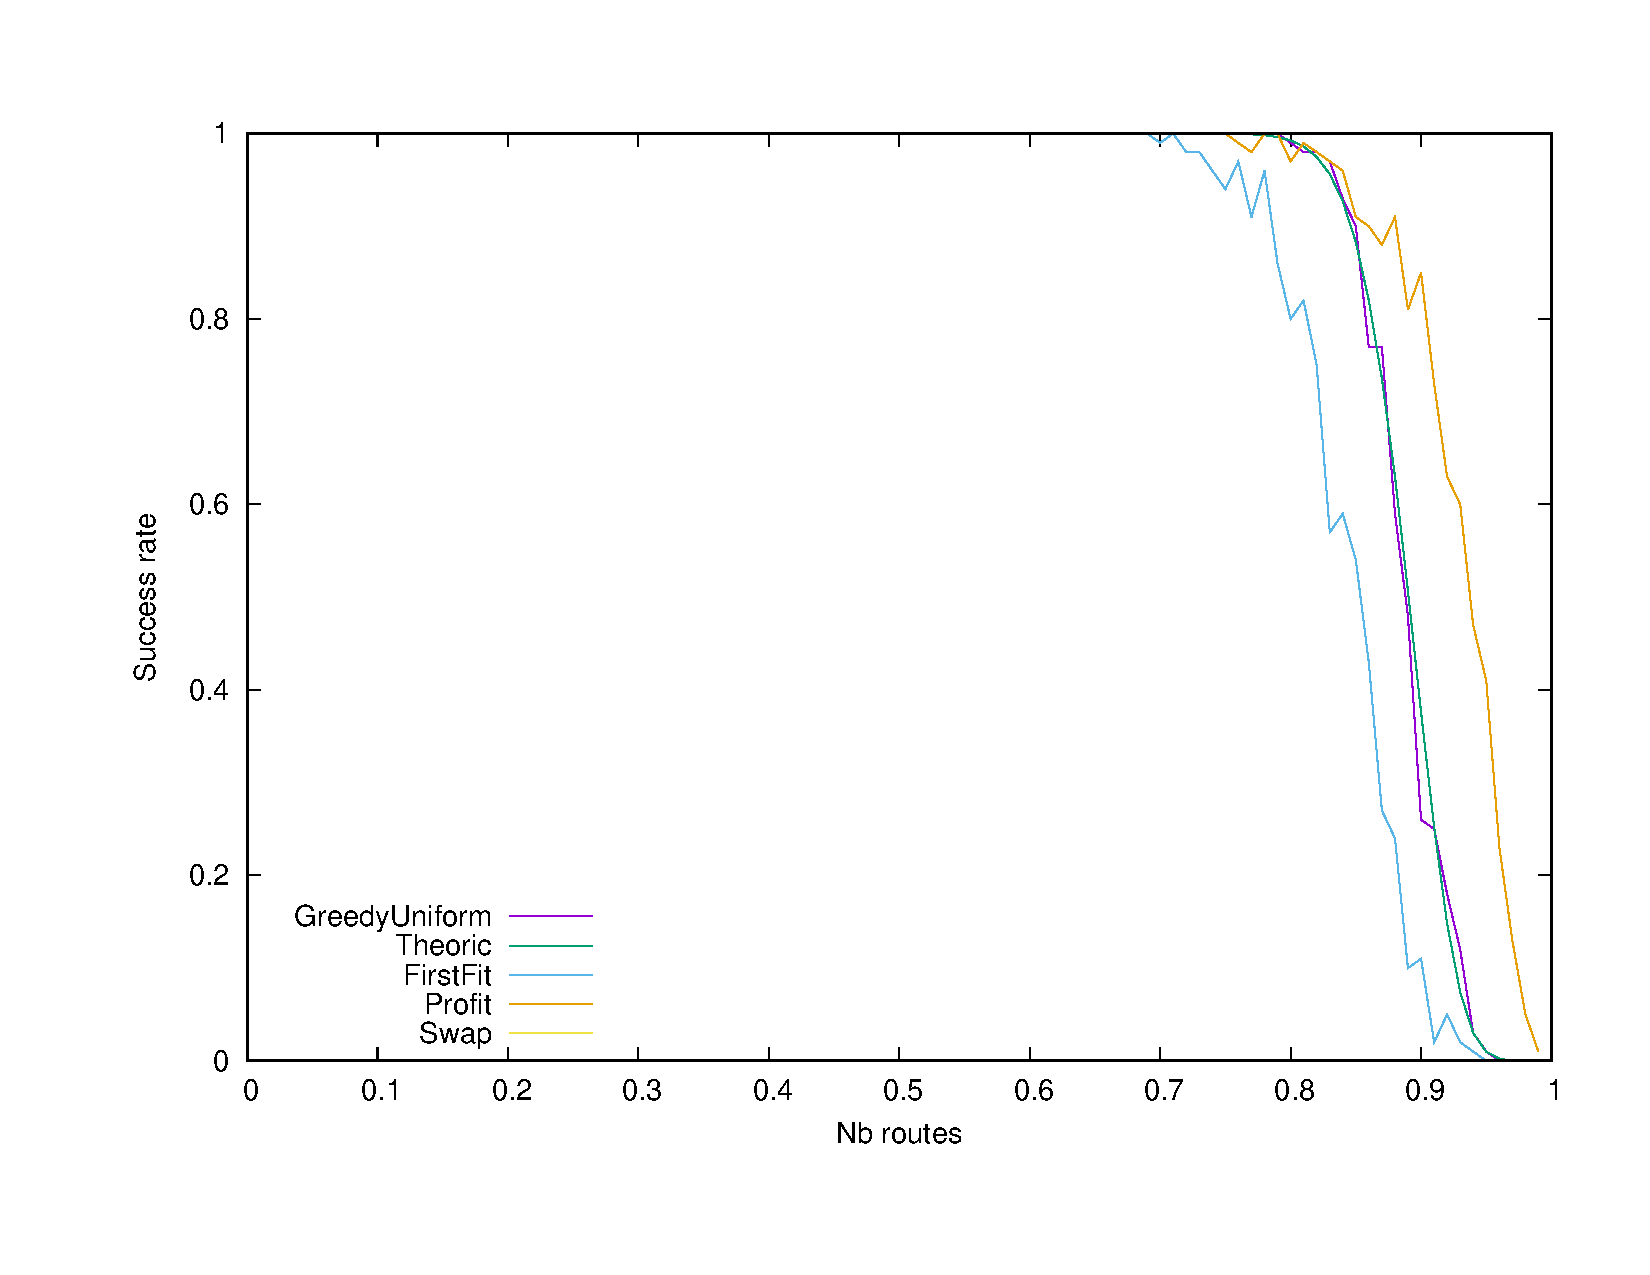
\includegraphics[scale=0.2]{success_tau1}
\end{center}
\caption{Success rate for $\tau = 1$ and $P=100$}
\label{fig:tau1}
\end{figure}




%\section{Lower bounds}

%Pour m=6, on peut toujours placer 5 éléments, que dire pour plus grand ?
%Remarque si tous les delais sont différents, on peut les placer, expliquer ça. 
%Example/family of examples for which some greedy alg fail -> facile pour le first fit
%Example/family of examples with a given load such that there are no feasible solution.

\bibliographystyle{ieeetr}
 \bibliography{Sources}

\end{document}
